\documentclass[12pt]{article}
\usepackage[utf8]{inputenc}
\usepackage[francais]{babel} 
\usepackage[T1]{fontenc}
\usepackage{amsmath}
\usepackage{amsfonts}
\usepackage{amssymb}
\usepackage{graphicx}
\usepackage{listings}
\usepackage{caption}
\usepackage{color}
\usepackage{xcolor}
\usepackage{lineno,amssymb}
\usepackage{array}
\usepackage{fancyhdr}
\usepackage{ifpdf}

\renewcommand{\floatpagefraction}{.999} 
\renewcommand{\textfraction}{.001}
\setcounter{totalnumber}{3} 

\definecolor{dkgreen}{rgb}{0,0.6,0}
\definecolor{gray}{rgb}{0.5,0.5,0.5}
\definecolor{mauve}{rgb}{0.58,0,0.90}

\DeclareCaptionFont{white}{\color{white}}
\DeclareCaptionFormat{listing}{\colorbox{gray}{\parbox{\textwidth}{#1#2#3}}}
\captionsetup[lstlisting]{format=listing,labelfont=white,textfont=white}
\renewcommand{\captionfont}{\small}
\setlength{\captionmargin}{13pt}
\setlength{\belowcaptionskip}{10pt}
\setlength{\abovecaptionskip}{10pt}

%\usepackage[left=2cm,right=2cm,top=2cm,bottom=2cm]{geometry}

\lstset{%
%frame=tRBl,
numbers=left,
numberstyle=\tiny,
frameround=tttt,
basicstyle=\footnotesize,%\sffamily,
captionpos=t,
stringstyle=\ttfamily,
backgroundcolor=\color{gray!5},
rulecolor=\color{black!30},
%inputencoding=utf8,
extendedchars=\true,%
showspaces=false,               % show spaces adding particular underscores
showstringspaces=false,         % underline spaces within strings
showtabs=false,                 % show tabs within strings adding particular underscores
keywordstyle=\color{blue},          % keyword style
commentstyle=\color{dkgreen},       % comment style
stringstyle=\color{mauve},         % string literal style
tabsize=2,
frame=trbl,
frameround=ffff,
xrightmargin=0pt,
%framexbottommargin=5pt,
xleftmargin=0pt,
columns=fullflexible,
basewidth=0.50em,
fontadjust=false,
lineskip=0pt,
xleftmargin=0pt,
framexleftmargin=0pt,
framexrightmargin=0pt,
framexbottommargin=3pt,
framextopmargin=3pt,
%inputencoding=utf8/latin1,%
literate={à}{{\`{a}}}2 {ê}{{\^{e}}}1 {è}{{\`{e}}}1 {ï}{{\¨{i}}}1 {ë}{{\¨{e}}}1 {î}{{\^{i}}}1 {é}{{\'{e}}}1 {ç}{{\c{c}}}1 {Ç}{{\c{C}}}1%
}

\ifpdf%
\usepackage[%
  pdfauthor={Alain Plantec},%
  pdfsubject={Méta-modélisation, vérification et validation : une approche outillées par l'orienté données},%
  pdftitle={Méta-modélisation, vérification et validation : une approche outillées par l'orienté données},%
  pdfkeywords={},%
  pdfstartview=FitH,%
  bookmarks=true,%
  bookmarksopen=true,%
  breaklinks=true,%
  colorlinks=true,%
  linkcolor=blue,anchorcolor=blue,%
  citecolor=blue,filecolor=blue,%
  menucolor=blue,%
  urlcolor=blue]{hyperref}
\else
\usepackage[%
  breaklinks=true,%
  colorlinks=true,%
  linkcolor=blue,anchorcolor=blue,%
  citecolor=blue,filecolor=blue,%
  menucolor=blue,%
  urlcolor=blue]{hyperref}
\fi

\lstdefinelanguage{express}
{keywords={ABS,ABSTRACT,ACOS,AGGREGATE,ALIAS,AND,ANDOR,ARRAY,
	AS,ASIN,ATAN,BAG,BEGIN,BINARY,BLENGTH,BOOLEAN,BY,
	CASE,CONST_E,CONSTANT,CONTEXT,COS,DERIVE,DIV,ELSE,
	END,END_ALIAS,END_CASE,END_CONSTANT,END_CONTEXT,END_ENTITY,
	END_FUNCTION,END_IF,END_LOCAL,END_MODEL,END_PROCEDURE,END_REPEAT,
	END_RULE,END_SCHEMA,END_TYPE,ENTITY,ENUMERATION,ESCAPE,EXISTS,
	EXP,FIXED,FOR,FORMAT,FROM,FUNCTION,GENERIC,HIBOUND,HIINDEX,
	IF,IN,INSERT,INTEGER,INVERSE,LENGTH,LIKE,LIST,LOBOUND,LOCAL,
	LOG,LOG10,LOG2,LOGICAL,LOINDEX,META, MOD,MODEL,NOT,NUMBER,NVL,
	ODD,OF,ONEOF,OPTIONAL,OR,OTHERWISE,PI,PROCEDURE,QUERY,REAL,
	REFERENCE,REMOVE,REPEAT,RETURN,ROLESOF,RULE,SCHEMA,SELECT,
	SELF,SET,SIN,SIZEOF,SKIP,SQRT,STRING,SUBTYPE,SUPERTYPE,
	TAN,THEN,TO,TYPE,TYPEOF,UNIQUE,UNTIL,USE,USEDIN,VALUE,
	VALUE_IN,VALUE_UNIQUE,VAR,WHERE,WHILE,XOR},
sensitive=f,
morestring=[d]",
morestring=[d]',
morecomment=[s]{(*}{*)},
morecomment=[l]--
}[keywords,comments,strings]

\author{Alain Plantec}

\title{Génération de code et interopérabilité\\Seconde partie}
\begin{document}
\thispagestyle{empty}
\maketitle

\tableofcontents
\pagebreak
La première partie a concerné la mise en oeuvre de \textit{minispec}, un langage de modélisation de données. Un modèle de données décrit avec \textit{minispec} peut servir de spécification source à différents outils. Pendans la première partie, un générateur de code vers Java a été développé.
Dans cette seconde partie, nous allons spécialiser minispec pour mettre en oeuvre un langage de modélisation de réseaux de capteurs.

\section{Réutilisation de \textit{minispec} pour mettre en oeuvre un langage spécialisé pour les réseaux de capteurs}
Nous allons développer un langage pour définir et programmer le comportement d'un réseaux de capteurs sans fils.
Un tel capteur est programmable par un script.
Un capteur est capable d'emettre et de recevoir des données de température et des données de localisation. 
Lorsqu'une donnée est émise, une led verte est allumée. Lors de la réception, une led rouge est allumée.


%\begin{figure}
%\begin{lstlisting}[language=express]
%entity Satellite ;
%  nom: String ;
%  id:Integer ;
%end_entity ;
%\end{lstlisting}
%\caption{Un exemple de specification avec \textit{minispec}}
%\label{fig:exemple-minispec1}
%\end{figure} 
%
%\begin{figure}
%\begin{center}
%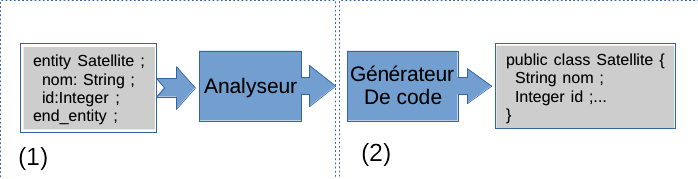
\includegraphics[scale=0.5]{generation-code-1.png}
%\end{center}
%\caption{Mise en oeuvre classique d'une génération de code}
%\label{fig:generation-code-1}
%\end{figure} 


\end{document}